\chapter{Object recognition emulation through neural networks}


\section{Convolutional neural networks}
\marginnote{Convolutional neural networks}

Deep convolutional neural networks (DCNNs) show an internal feature representation similar to the representation of the ventral pathway (primate ventral visual stream).
Moreover, object confusion in DCNNs is similar to the behavioral patterns in primates.

However, on a higher resolution level (i.e. not object but image level), the performance of DCNNs diverges drastically from human behavior.

\begin{remark}
    Studies using HCNN have also been presented in the previous chapter.
\end{remark}

\begin{casestudy}[Humans and monkeys object confusion \cite{human_monkey_confusion}]
    It has been seen that monkeys show a confusion pattern correlated to that of humans on the task of object recognition.
    Convolutional neural networks also show this correlation while low-level visual representations (V1 or pixels, a baseline computed from the pixels of the image)
    correlate poorly.
    \begin{figure}[H]
        \centering
        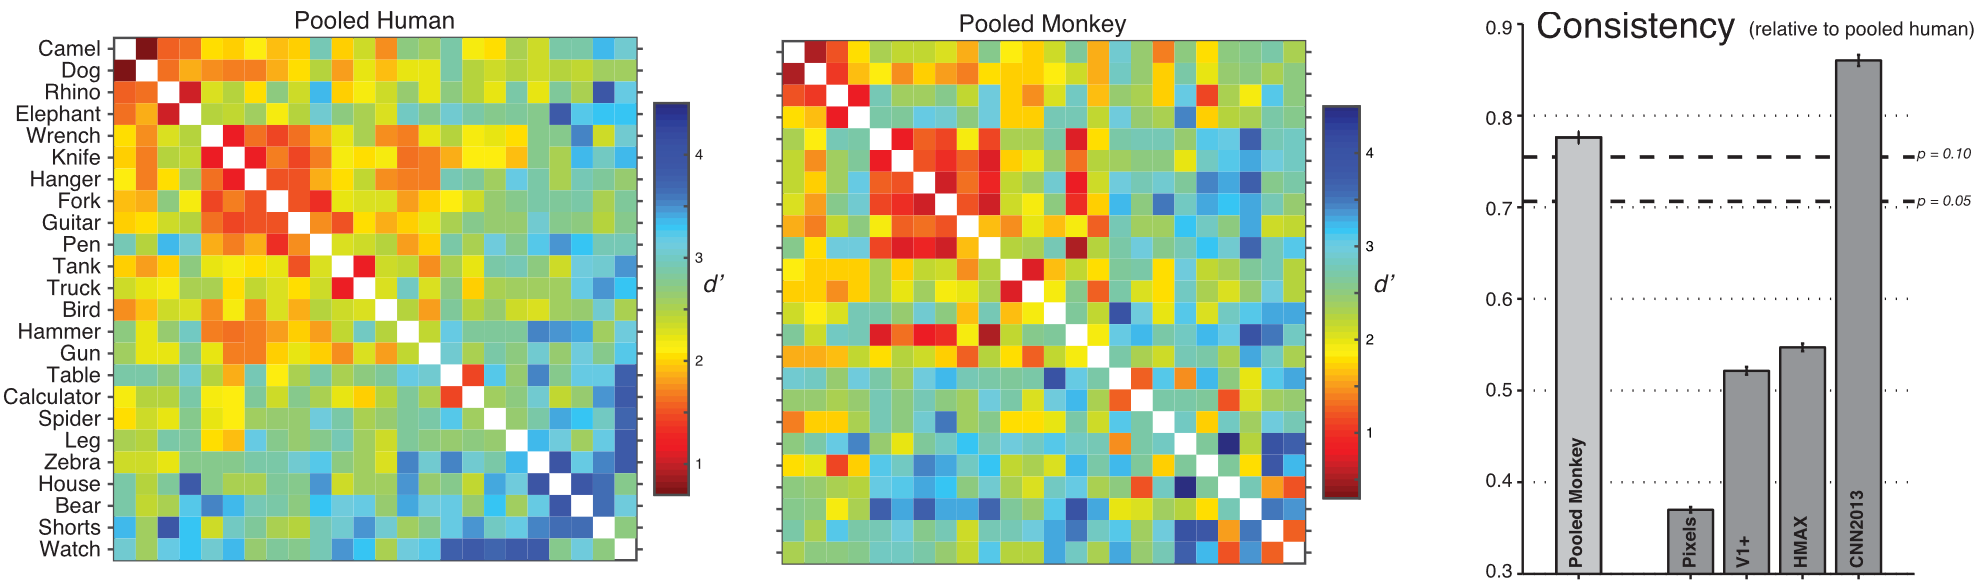
\includegraphics[width=0.8\linewidth]{./img/human_monkey_confusion.png}
    \end{figure} 
\end{casestudy}

\begin{casestudy}[Primates and DCNNs object recognition divergence \cite{human_dcnn_divergence}]
    Humans, monkeys and DCNNs are trained for the task of object recognition.

    To enforce an invariance recognition behavior, each image has an object with a random transformation (position, rotation, size)
    and has a random natural background.

    \begin{figure}[H]
        \centering
        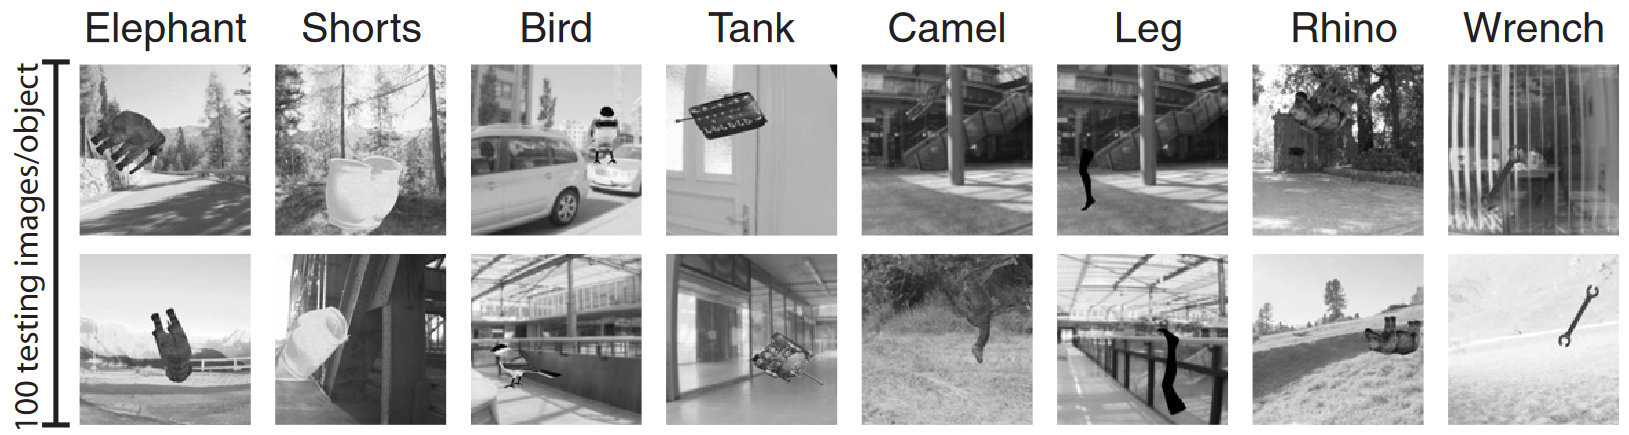
\includegraphics[width=0.65\linewidth]{./img/human_dcnn_divergence3.png}
    \end{figure}

    \begin{itemize}
        \item For humans, a trial starts with fixation. Then, an image is displayed for 100 ms followed by a binary choice.
            The human has to make its choice in 1000 ms.
    
        \item For monkeys, a trial starts with fixation. Then, an image is displayed for 100 ms followed by a binary choice.
            The monkey has up to 1500 ms to freely view the response images and has to maintain fixation on its choice for 700 ms.
        
        \item DCNNs are trained as usual.
    \end{itemize}

    \begin{figure}[H]
        \centering
        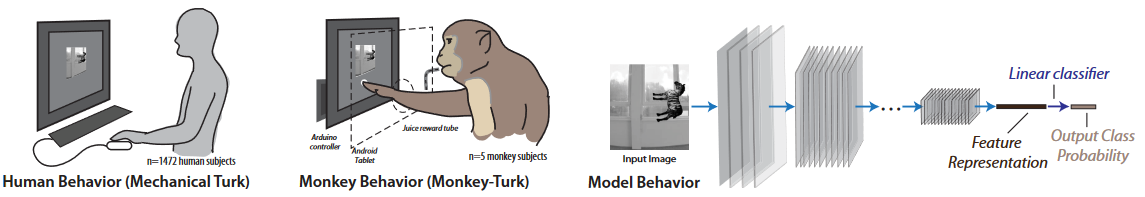
\includegraphics[width=0.85\linewidth]{./img/human_dcnn_divergence1.png}
    \end{figure}

    \begin{figure}[H]
        \centering
        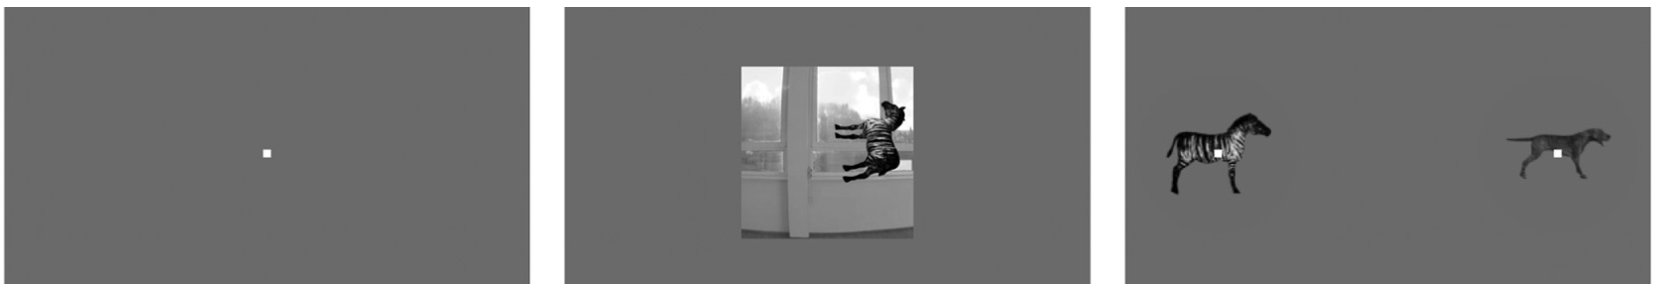
\includegraphics[width=0.7\linewidth]{./img/human_dcnn_divergence2.png}
        \caption{Steps of a trial}
    \end{figure}

    Performance is measured using behavioral metrics.
    Results show that:
    \begin{descriptionlist}
        \item[Object-level] 
            Object-level measurements are obtained as an average across all images of that object.

            Recognition confusion of primates and DCNNs are mostly correlated.

            \begin{figure}[H]
                \centering
                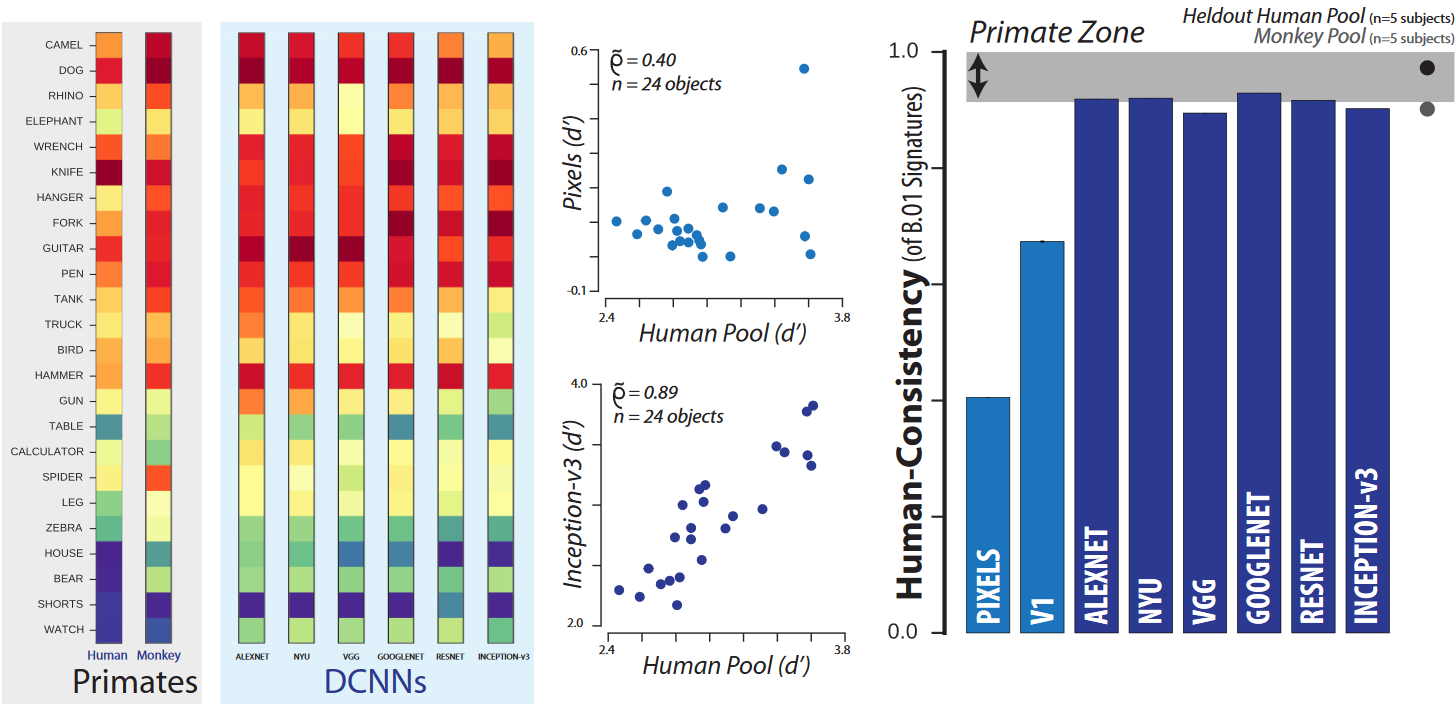
\includegraphics[width=0.65\linewidth]{./img/human_dcnn_divergence4.png}
                \caption{
                    \parbox[t]{0.6\linewidth}{
                        Object-level results. In the first part, warmer colors indicate a better classification.
                    }
                }
            \end{figure}

        \item[Image-level] 
            Image-level measurements are obtained by normalizing the raw classification results.

            All DCNNs fail to replicate the behavioral signatures of primates.
            This hints at the fact that the architecture and/or the training process is limiting the capability of the models.

            \begin{figure}[H]
                \centering
                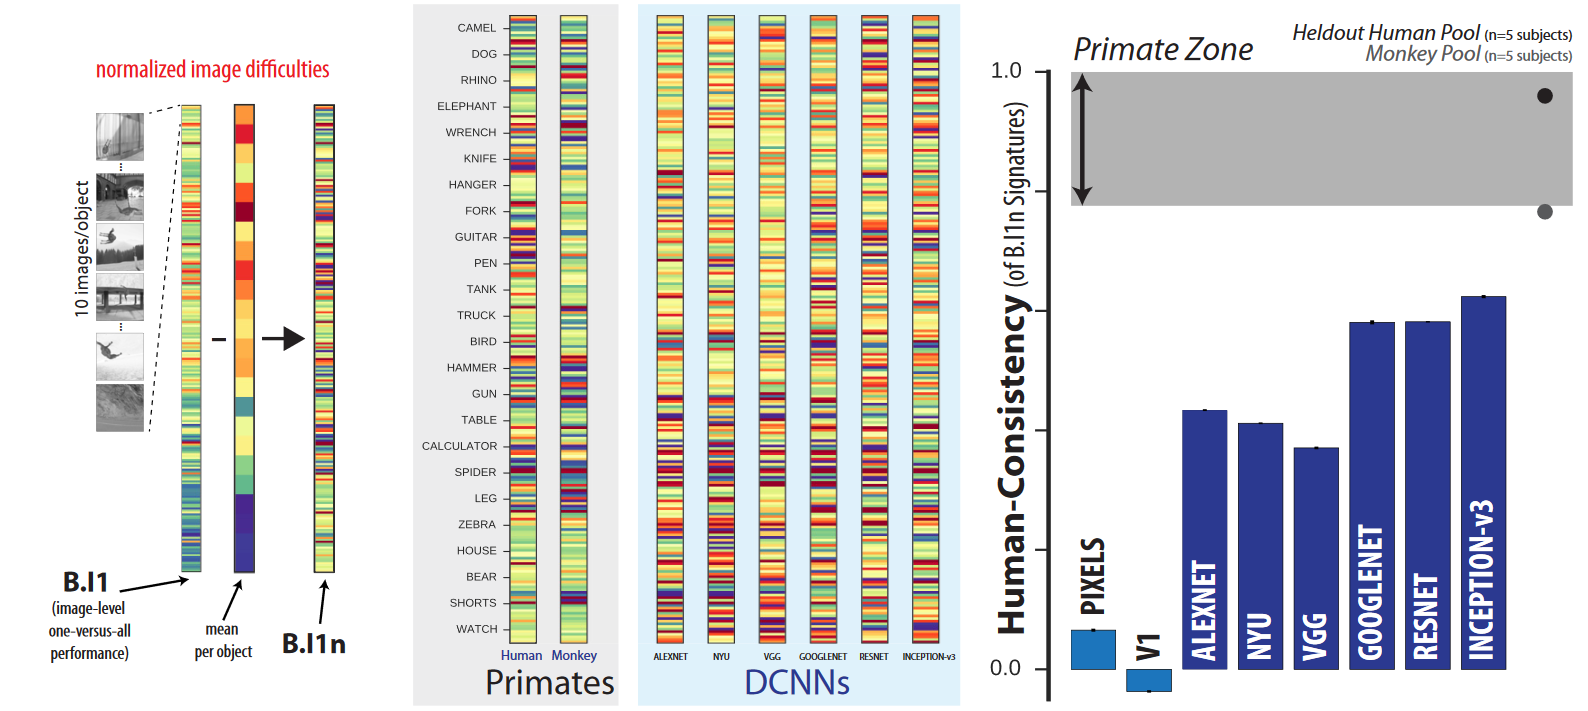
\includegraphics[width=0.75\linewidth]{./img/human_dcnn_divergence5.png}
            \end{figure}
    \end{descriptionlist}
\end{casestudy}



\section{Recurrent neural networks}
\marginnote{Recurrent neural networks}


\subsection{Object recognition}

The short duration for which candidates of the previous experiments were exposed to an image 
suggests that recurrent computation is not relevant for core object recognition.
However, the following points are in contrast with this hypothesis:
\begin{itemize}
    \item DCNNs fail to predict primate behavior in many cases.
    \item Specific image instances (e.g. blurred, cluttered, occluded) are easy for primates but difficult for DCNNs.
\end{itemize}
This hints at the fact that recurrent computation might be involved, maybe at later stages of the recognition process.

\begin{casestudy}[Primates recognition reaction time \cite{recognition_reaction}]
    \phantom{}
    \begin{descriptionlist}
        \item[Recognition training and evaluation] 
            Humans, macaques and DCNNs are trained for the task of object recognition on
            images with two levels of difficulty:
            \begin{descriptionlist}
                \item[Control images] Easier to recognize.
                \item[Challenge images] Harder to recognize.
            \end{descriptionlist}
            Results show that primates outperform DCNNs on challenge images.
        
            \begin{figure}[H]
                \centering
                \begin{subfigure}{0.6\linewidth}
                    \centering
                    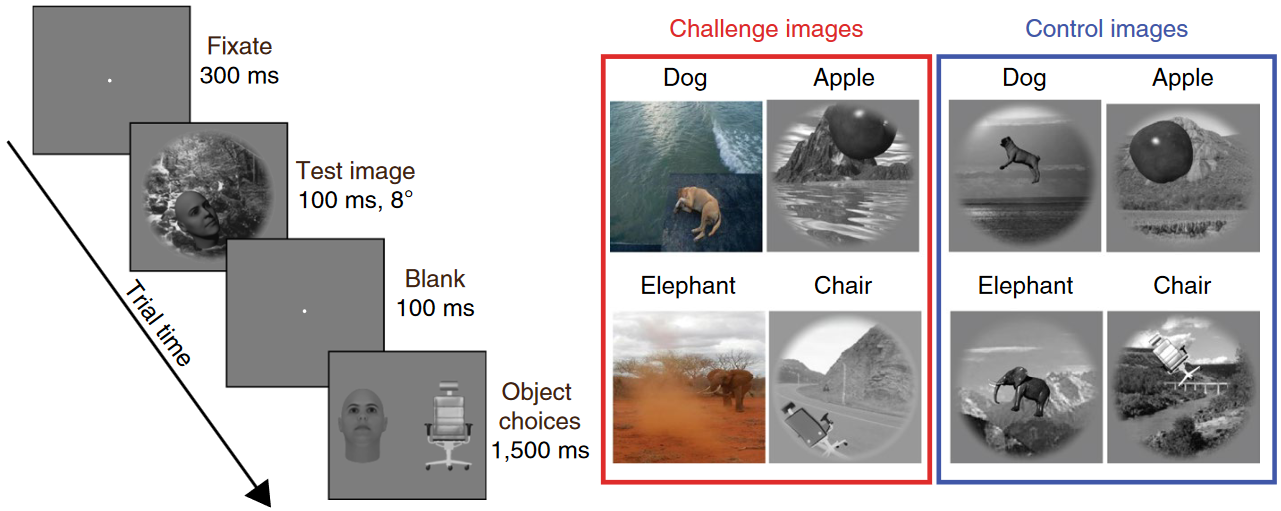
\includegraphics[width=\linewidth]{./img/recognition_reaction1.png}
                \end{subfigure}
                \begin{subfigure}{0.25\linewidth}
                    \centering
                    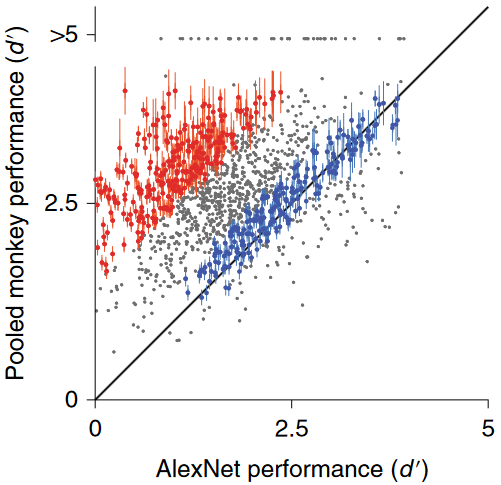
\includegraphics[width=\linewidth]{./img/recognition_reaction2.png}
                \end{subfigure}
                \caption{
                    \parbox[t]{0.7\linewidth}{
                        Trial steps, example images and behavioral comparison between monkeys and DCNNs. 
                        Red and blue points in the graph are challenge and control images, respectively.
                    }
                }
            \end{figure}

        \item[Reaction time]
            It also has been observed that the reaction time of both humans and monkeys for challenge images is significantly higher than the reaction for control images
            ($\Delta\text{RT} = 11.9 \text{ ms}$ for monkeys and $\Delta\text{RT} = 25 \text{ ms}$ for humans).
        
            To determine the time at which the identity of an object is formed in the IT cortex, 
            the neural activity is measured every 10 ms after the stimulus onset and a linear classifier (decoder) is trained to determine the \textbf{neural decode accuracy (NDA)}
            (i.e. the best accuracy that the classifier can achieve with the information in that time slice).
            We refer with \textbf{object solution time (OST)} the time at which the NDA reached the primate accuracy (i.e. high enough).
        
            It has been observed that challenge images have a slightly higher OST ($\sim 30 \text{ ms}$) 
            whether the animal was actively performing the task or passively viewing the image.
            \begin{figure}[H]
                \centering
                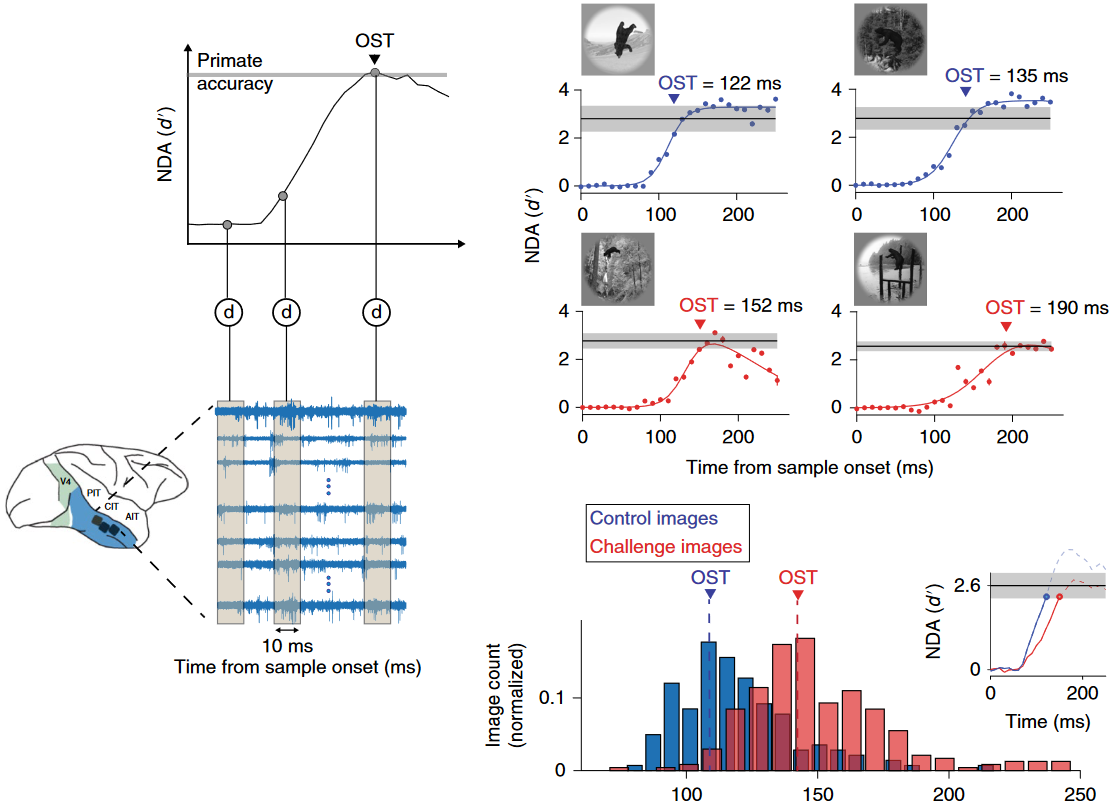
\includegraphics[width=0.7\linewidth]{./img/recognition_reaction3.png}
            \end{figure}

        \item[DCNN IT prediction]
            The IT neuronal response for a subset of challenge and control images has been measured across 10 ms bins
            to obtain two sets $R^\text{train}$ and $R^\text{test}$ (50/50).
            
            During training, the activation $F^\text{train}$ of a layer of the DCNN is used to predict $R^\text{train}$ 
            through partial least square regression (i.e. a linear combination of $F^\text{train}$).

            During testing, the activation of the same layer of the DCNN is transformed using the found parameters and compared to $R^\text{test}$.

            Results show a higher predictivity for early responses (which are mainly feed-forward) and a significant drop over time.
            The drop coincides with the OST of challenge images, hinting at the fact that later phases of the IT might involve recurrence.
            \begin{figure}[H]
                \centering
                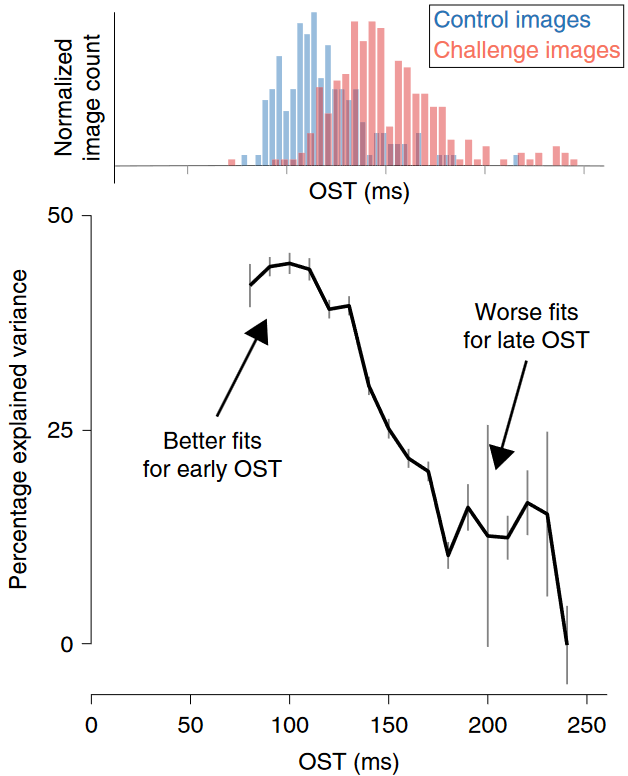
\includegraphics[width=0.35\linewidth]{./img/recognition_reaction4.png}
            \end{figure}

        \item[CORnet IT prediction]
            The previous experiment has also been done using deeper CNNs that showed better predictivity.
            This can be explained by the fact that deeper networks simulate the unrolling of a recurrent network and are therefore an approximation of them.

            Deeper networks are also able to solve some of the challenge images but those that remained unsolved
            are those with the longest OSTs among the challenge images.

            CORnet, a four-layer recurrent neural network, has also been experimented.
            Results show that the first layers of CORnet are good predictors of the early IT phases while the last layers are good at predicting the late phases of IT.

            \begin{figure}[H]
                \centering
                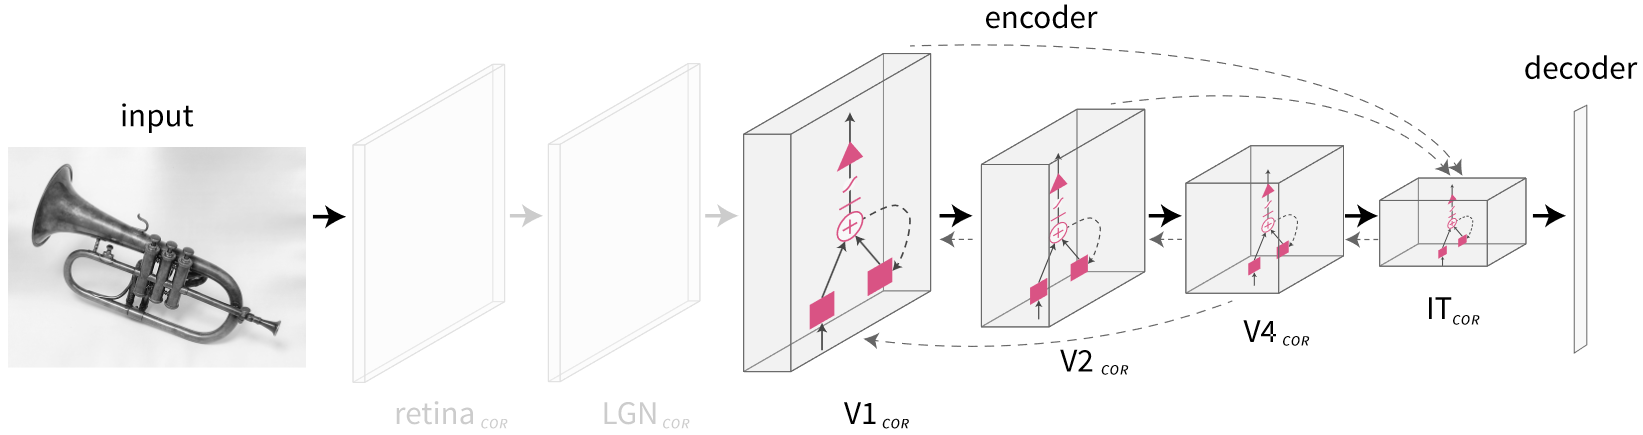
\includegraphics[width=0.7\linewidth]{./img/cornet.png}
                \caption{Architecture of CORnet}
            \end{figure}

            \begin{figure}[H]
                \centering
                \begin{subfigure}{0.48\linewidth}
                    \centering
                    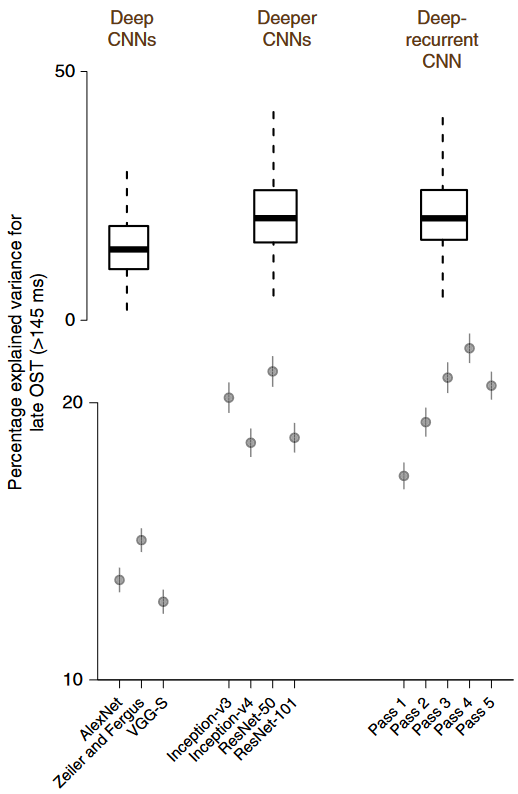
\includegraphics[width=0.6\linewidth]{./img/recognition_reaction5.png}
                    \caption{
                        \parbox[t]{0.9\linewidth}{
                            Predictivity for deep, deeper and recurrent CNNs
                        }
                    }
                \end{subfigure}
                \begin{subfigure}{0.48\linewidth}
                    \centering
                    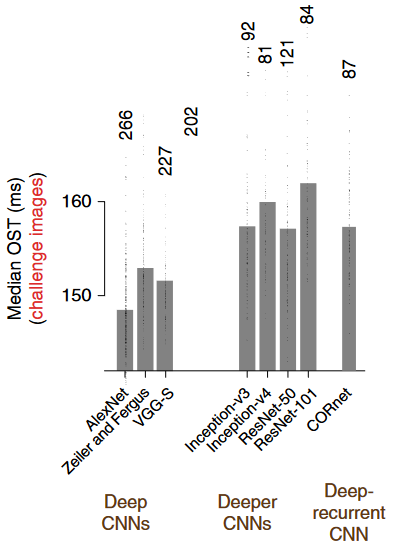
\includegraphics[width=0.6\linewidth]{./img/recognition_reaction6.png}
                    \caption{
                        \parbox[t]{0.9\linewidth}{
                            Number (on top) and median OST (bars) of the unsolved images for each model
                        }
                    }
                \end{subfigure}
            \end{figure}

            \begin{remark}
                Recurrence can be seen as additional non-linear transformations in addition to those of the feed-forward phase.
            \end{remark}
    \end{descriptionlist}
\end{casestudy}


\subsection{Visual pattern completion}


\begin{description}
    \item[Pattern completion] \marginnote{Pattern completion}
        Ability to recognize poorly visible or occluded objects.

        \begin{remark}
            The visual system is able to infer an object even if only 10-20\% of it is visible.

            It is hypothesized that recurrent computation is involved.
        \end{remark}
\end{description}

\begin{casestudy}[Human and RNN pattern completion \cite{pattern_completion}]
    \phantom{}
    \begin{descriptionlist}
        \item[Trial structure] 
            Whole and partial images are presented to humans through two types of trials:
            \begin{descriptionlist}
                \item[Unmasked] 
                    After fixation, an image is displayed for a short time followed by a blank screen. Then, a response is required from the candidate.
        
                \item[Backward masking] 
                    After fixation, an image is displayed for a short time followed by another image. Then, a response is required from the candidate.
                    The second image aims to interrupt the processing of the first one (i.e. interrupt recurrent processing).
            \end{descriptionlist}
        
            \begin{figure}[H]
                \centering
                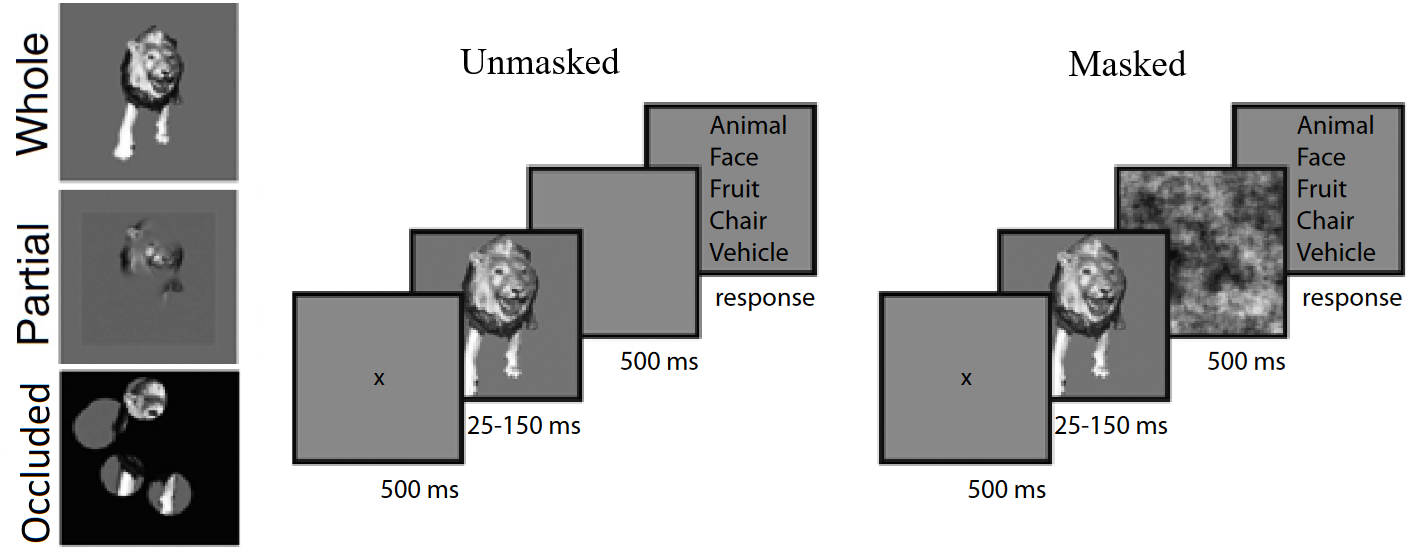
\includegraphics[width=0.55\linewidth]{./img/pattern_completion1.png}
            \end{figure}

        \item[Human results]
            Results show that subjects are able to robustly recognize whole and partial objects in the unmasked case.
            In the masked case, performances are instead worse.
            \begin{figure}[H]
                \centering
                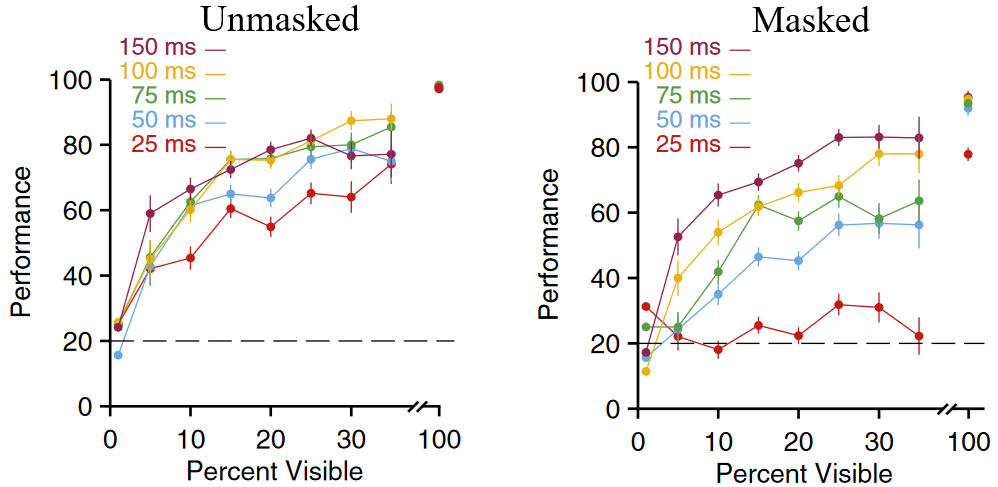
\includegraphics[width=0.5\linewidth]{./img/pattern_completion2.png}
            \end{figure}
        
            Moreover, measurements show that the neural response to partially visible objects is delayed compared to whole images, 
            hinting at the fact that additional computation is needed.
            \begin{figure}[H]
                \centering
                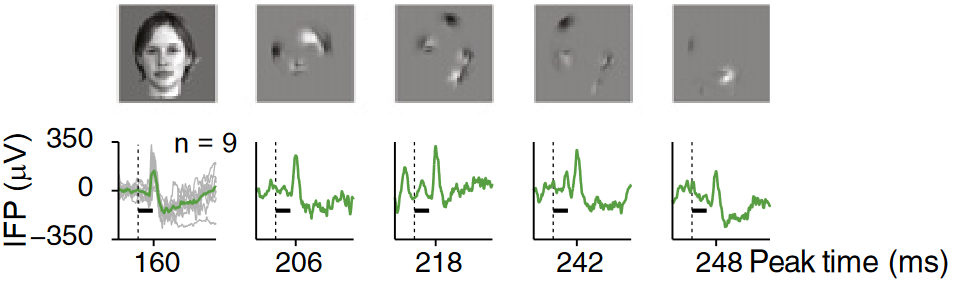
\includegraphics[width=0.5\linewidth]{./img/pattern_completion3.png}
                \caption{
                    Activity (IFP) of a neuron that responds to faces
                }
            \end{figure}

        \item[CNN results]
            Feed-forward CNNs have also been trained on the task of object recognition.
            \begin{itemize}
                \item Performances are comparable to humans for whole images but decline for partial images.
                \item There is a slight correlation between the latency of humans' neural response and 
                    the distance of the internal representation in the CNNs of each partial object to its whole image.
            \end{itemize}
        
            \begin{figure}[H]
                \centering
                \begin{subfigure}{0.33\linewidth}
                    \centering
                    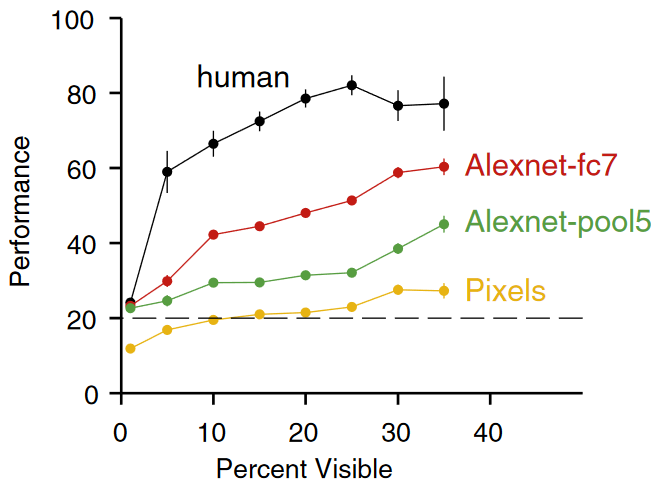
\includegraphics[width=0.9\linewidth]{./img/pattern_completion4.png}
                \end{subfigure}
                \begin{subfigure}{0.65\linewidth}
                    \centering
                    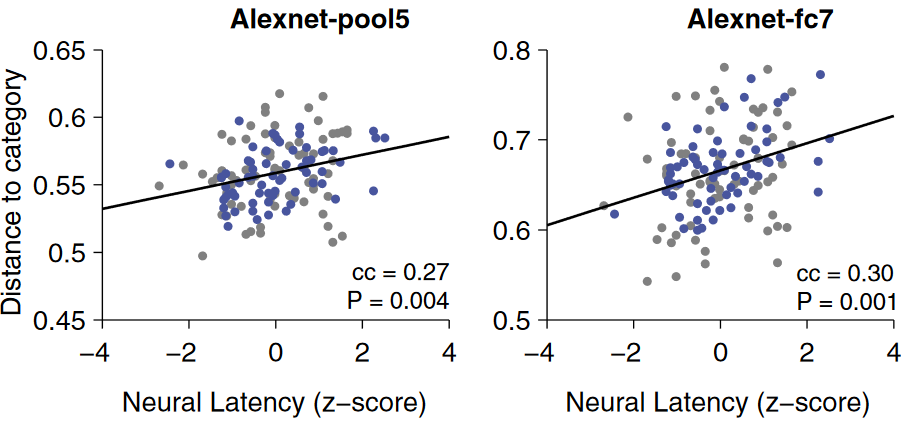
\includegraphics[width=0.6\linewidth]{./img/pattern_completion5.png}
                    \caption{Representation and latency correlation. The color of the dots depends on the electrode that measured the latency.}
                \end{subfigure}
            \end{figure}

        \item[RNN results]
            Recurrent neural networks have also been tested by using existing CNNs enhanced through attractor networks\footnote{
                Recurrent network with multiple attractor points each representing a whole image. 
                By processing the same partial image for multiple time steps, its representation should converge to an attractor point.
            } (Hopfield network, RNNh).
            Results show that RNNh has higher performance in pattern completion.
        
            \begin{figure}[H]
                \centering
                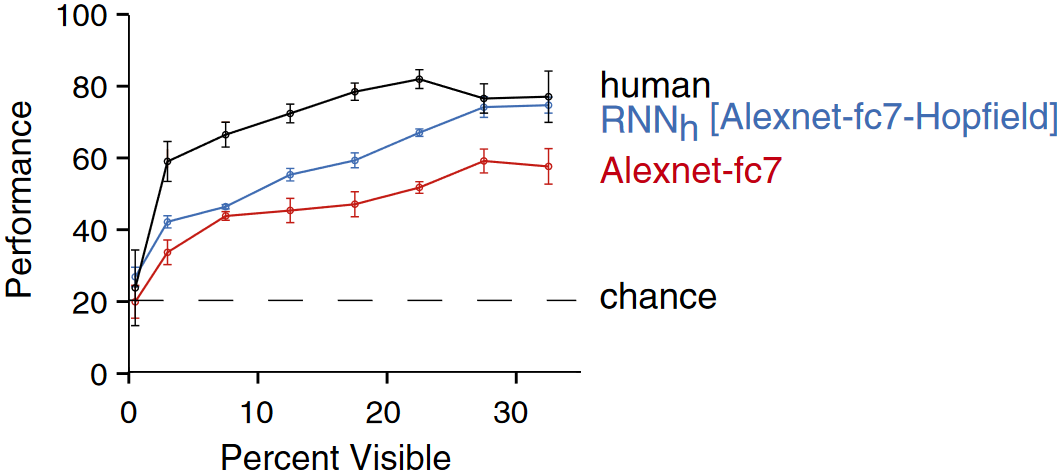
\includegraphics[width=0.45\linewidth]{./img/pattern_completion6.png}
            \end{figure}
        
            Moreover, by plotting the temporal evolution of the internal representation of partial objects, 
            it can be seen that, at the beginning, partial images are more similar among themselves than their corresponding attractor point,
            but, over time, their representation approaches the correct cluster.
            \begin{figure}[H]
                \centering
                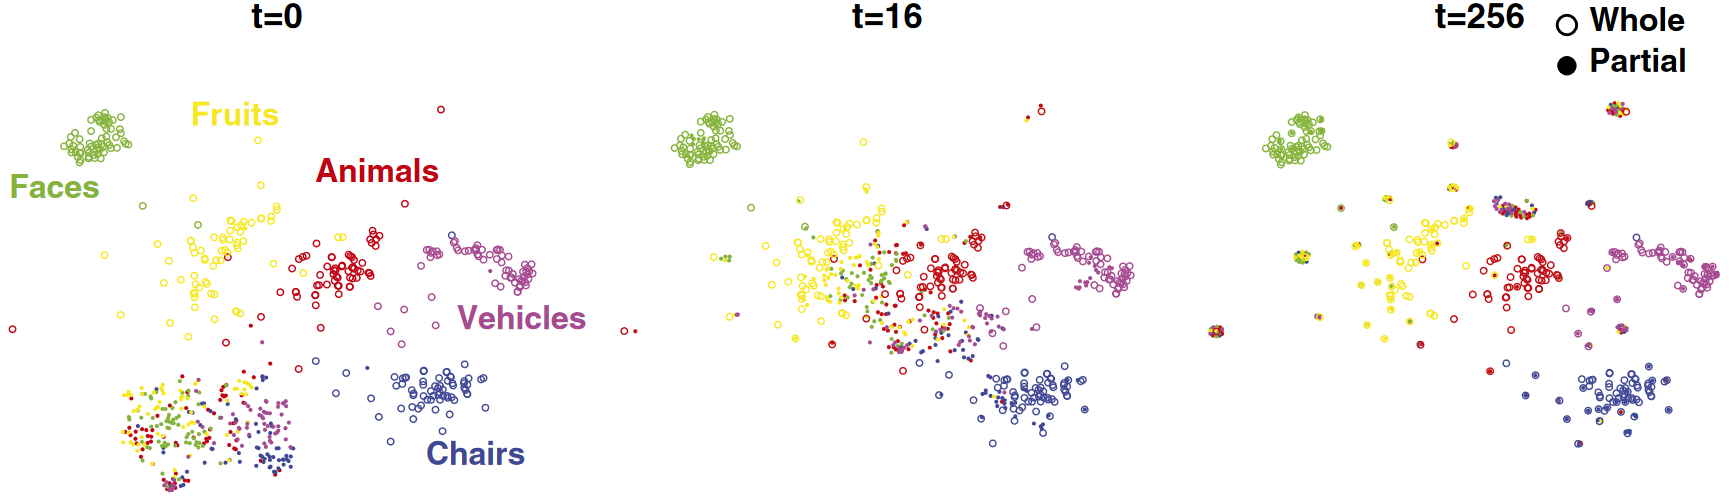
\includegraphics[width=0.7\linewidth]{./img/pattern_completion7.png}
            \end{figure}
        
            Time-wise, RNNh performance and correlation with humans increase over the time steps and saturates at around 10-20 steps.
            This is consistent with the physiological delays of the human ventral visual stream.
            \begin{figure}[H]
                \centering
                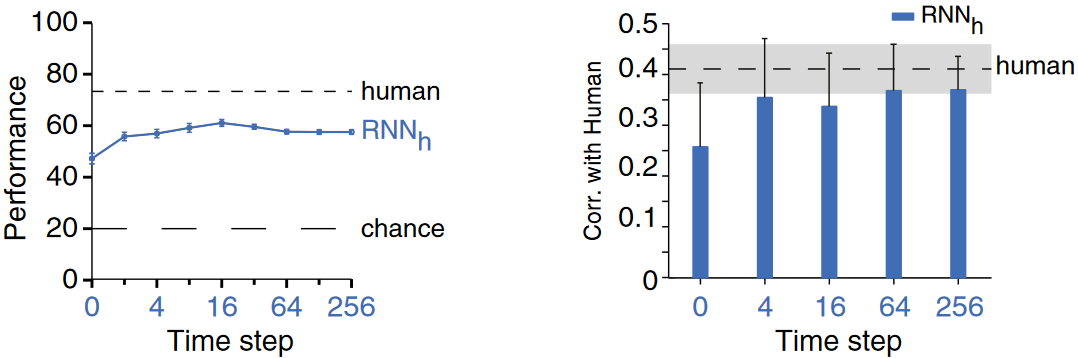
\includegraphics[width=0.55\linewidth]{./img/pattern_completion8.png}
            \end{figure}
        
            By backward masking the input of the RNNh (i.e. present the image for a few time steps and then change it), performance drops from $58 \pm 2\%$ to $37 \pm 2\%$.
            \begin{figure}[H]
                \centering
                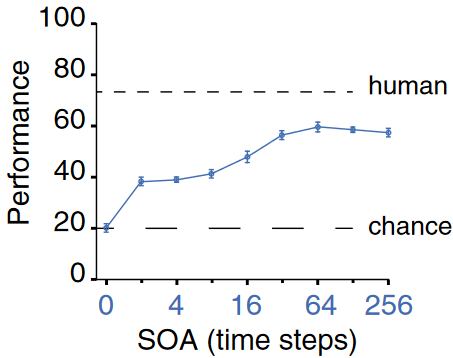
\includegraphics[width=0.25\linewidth]{./img/pattern_completion9.png}
            \end{figure}
    \end{descriptionlist}
\end{casestudy}



\section{Unsupervised neural networks}
\marginnote{Unsupervised neural networks}

Most of the models to simulate the visual cortex are trained on supervised datasets of millions of images.
Such supervision is not able to explain how primates learn to recognize objects as processing a huge amount of category labels during development is highly improbable.
Possible hypotheses are:
\begin{itemize}
    \item Humans might rely on different inductive biases for a more efficient learning.
    \item Humans might augment their initial dataset by combining known instances.
\end{itemize}

Unsupervised learning might explain what happens in between 
the representations at low-level visual areas (i.e. the retina), which are mostly hardcoded from evolution,
and the representations learned at higher levels.

\begin{figure}[H]
    \centering
    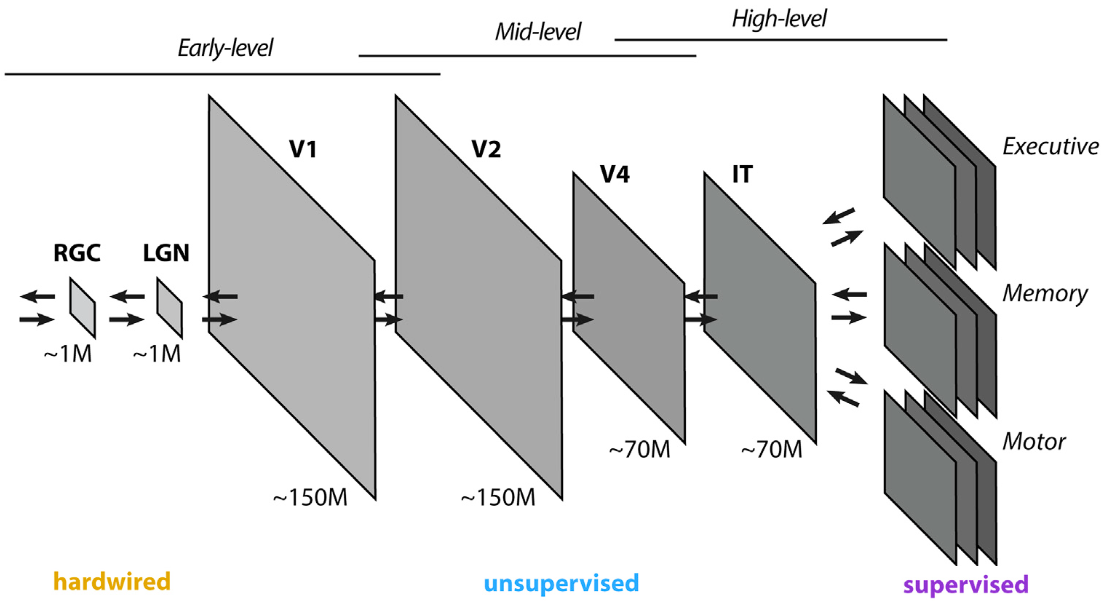
\includegraphics[width=0.55\linewidth]{./img/vision_learning_method.png}
\end{figure}

\begin{casestudy}[Unsupervised embedding \cite{unsupervised_embedding}]
    Different unsupervised embedding methods are used to create a representation for a dataset of images that are then assessed on various tasks.

    \begin{descriptionlist}
        \item[Contrastive embedding] 
            Unsupervised embedding method that uses a DCNN (which simulates low-level visual areas) to create the representation of an image in a low dimensional space and 
            then optimize it by pushing each embedding closer to its close neighbors and far from its background neighbors.
            \begin{figure}[H]
                \centering
                \begin{subfigure}{0.75\linewidth}
                    \centering
                    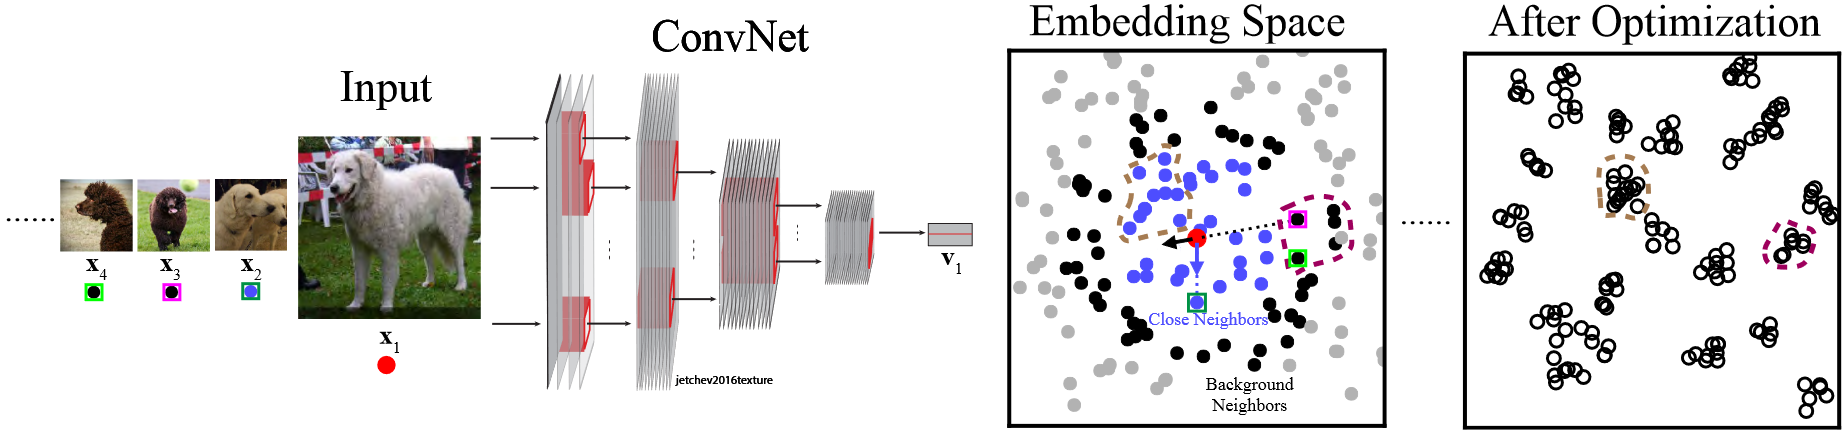
\includegraphics[width=\linewidth]{./img/local_aggregation1.png}
                \end{subfigure}
                \begin{subfigure}{0.55\linewidth}
                    \centering
                    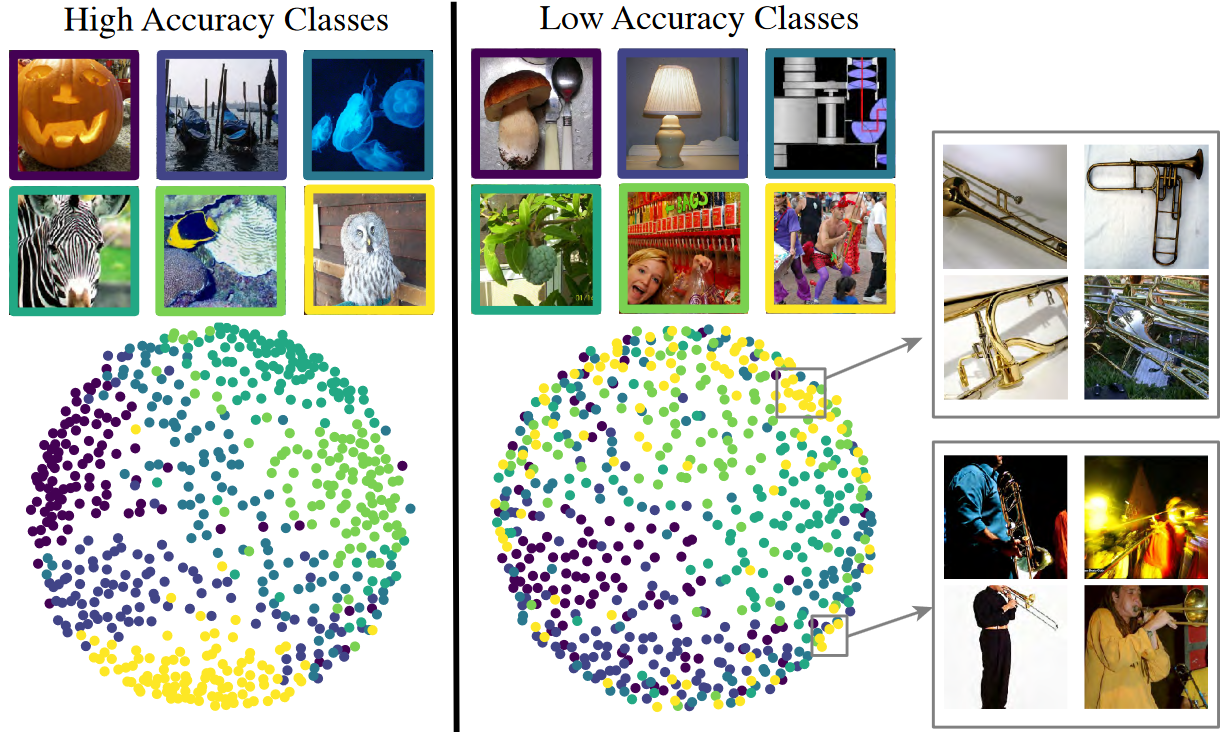
\includegraphics[width=\linewidth]{./img/local_aggregation2.png}
                \end{subfigure}
                \caption{Workflow and visualization of the local aggregation algorithm}
            \end{figure}

        \item[Results on object recognition tasks]
            To solve the tasks, unsupervised embeddings are used in conjunction with a linear classifier.
            A supervised DCNN is also used as a baseline.
            
            Results show that:
            \begin{itemize}
                \item Among all the unsupervised methods, contrastive embeddings have the best performances.
                \item Unsupervised methods equaled or outperformed the DCNN on tasks such as object position and size estimation.
                \item The DCNN outperforms unsupervised models on categorization tasks.
            \end{itemize} 

            \begin{figure}[H]
                \centering
                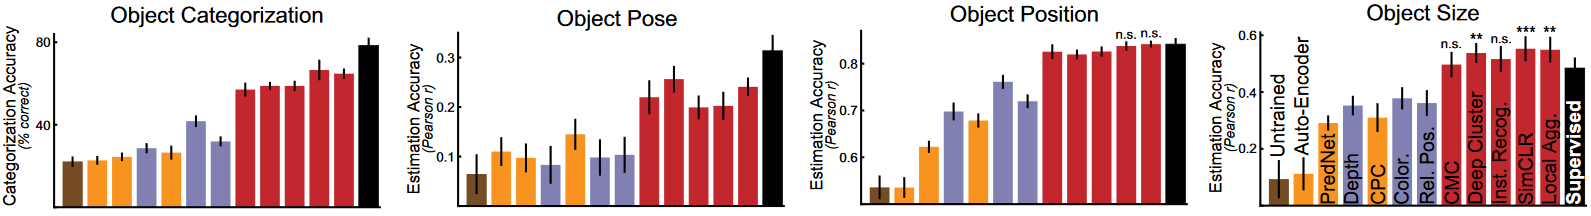
\includegraphics[width=0.95\linewidth]{./img/unsupervised_embedding1.png}
                \caption{
                    \parbox[t]{0.7\linewidth}{
                        Evaluation accuracy of an untrained model (brown), predictive encoding methods (orange), 
                        self-supervised methods (blue), contrastive embeddings (red) and a supervised DCNN (black). 
                    }
                }
            \end{figure}

        \item[Results on neural data]
            Techniques to map the responses of an artificial network to real neural responses have been used to evaluate unsupervised methods.

            Results show that:
            \begin{descriptionlist}
                \item[Area V1] None of the unsupervised methods are statistically better than the DCNN.
                \item[Area V4] A subset of methods equaled the DCNN.
                \item[Area IT] Only contrastive embeddings equaled the DCNN.
            \end{descriptionlist}

            \begin{figure}[H]
                \centering
                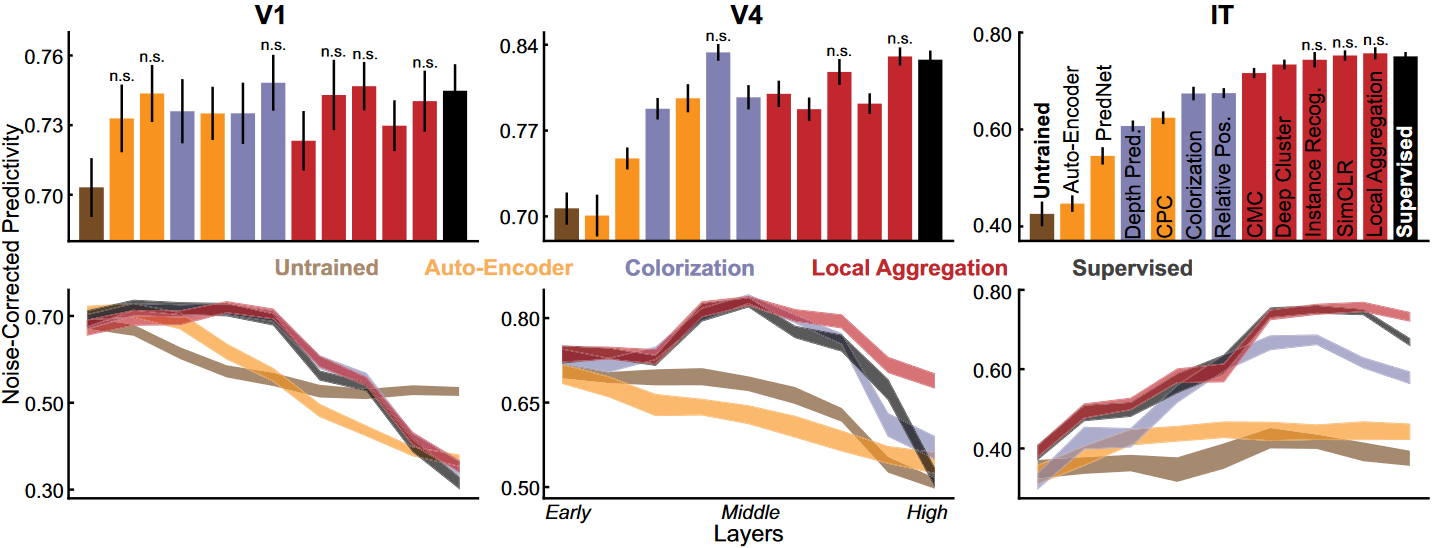
\includegraphics[width=0.8\linewidth]{./img/unsupervised_embedding2.png}
            \end{figure}
        
        \item[Results on video data]
            As training on single distinct images (ImageNet) is significantly different from real biological data streams,
            a dataset containing videos (SAYCam) has been experimented with.
            A contrastive embedding, the VIE algorithm, has been employed to predict neural activity.

            Results show that embeddings learned from videos are comparable to those learned from only images.

            \begin{figure}[H]
                \centering
                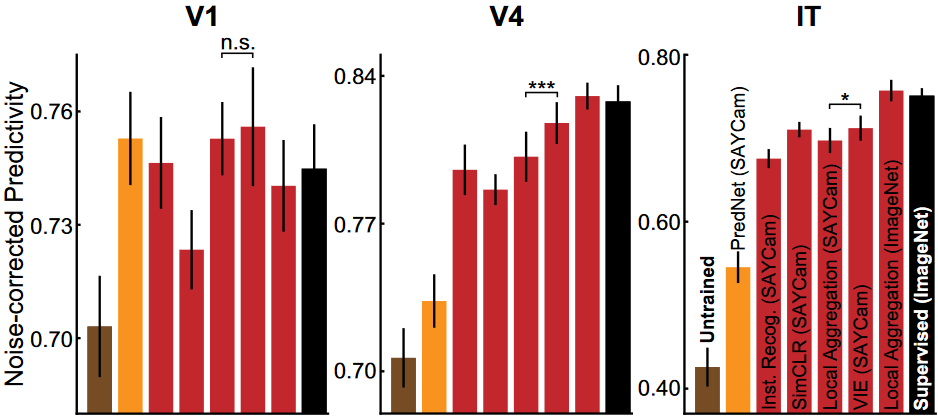
\includegraphics[width=0.6\linewidth]{./img/unsupervised_embedding3.png}
            \end{figure}

        \item[Semi-supervised learning]
            Semi-supervised embedding aims to find a representation using a small subset of labeled data points and a large amount of unlabeled data.

            \begin{figure}[H]
                \centering
                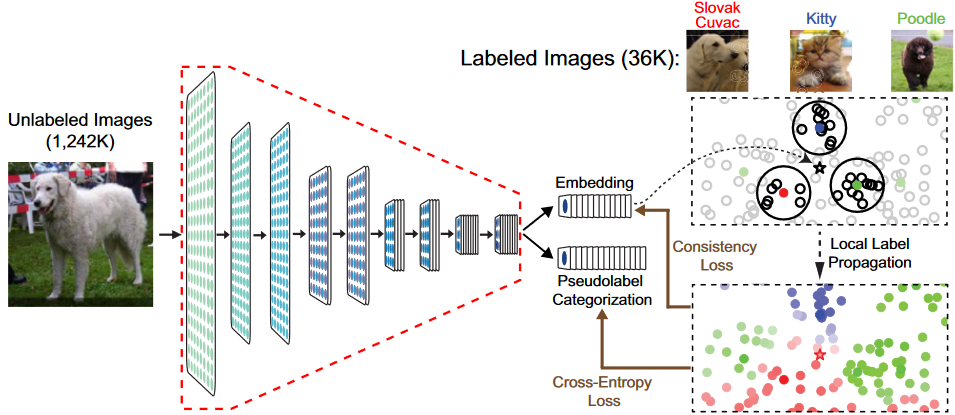
\includegraphics[width=0.75\linewidth]{./img/local_label_propagation.png}
                \caption{Workflow of the local label propagation algorithm}
            \end{figure}

            Results show that semi-supervised embeddings with only a $3\%$ of supervision are substantially more consistent than purely unsupervised methods.
            Although, the gap between them and the DCNN still remains.

            Nevertheless, a significant gap is also present between the results of all the models and the noise ceiling of the data, 
            indicating that there still are inconsistencies between artificial networks and the human visual system.

            \begin{figure}[H]
                \centering
                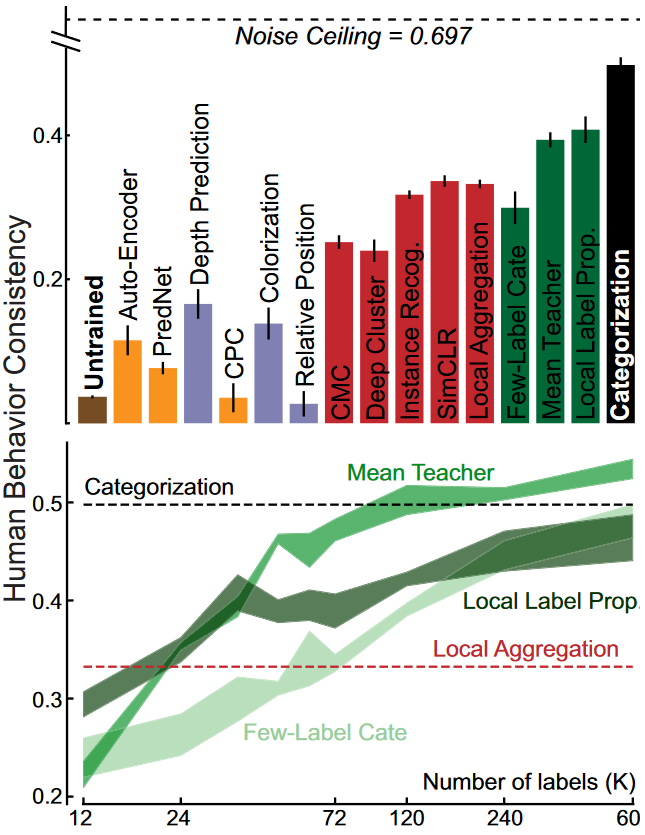
\includegraphics[width=0.40\linewidth]{./img/unsupervised_embedding4.png}
            \end{figure}
    \end{descriptionlist}
\end{casestudy}